% This example An LaTeX document showing how to use the l3proj class to
% write your report. Use pdflatex and bibtex to process the file, creating 
% a PDF file as output (there is no need to use dvips when using pdflatex).

% Modified 

\documentclass{l3proj}
\begin{document}
\title{Team V - How Not To Kill Your Dog}
\author{Ross Adam \\
        Andrew Gardner \\
        Nicole Kearns \\
        Mamas Nicolaou \\
        Asset Sarsengaliyev}
\date{18 March 2013}
\maketitle
\begin{abstract}

The abstract goes here

\end{abstract}
\educationalconsent
\tableofcontents

\chapter{Background}
\label{background}

\section{Investigation of Existing Artifacts}


There are a few similar tools and learning resources available for vetinary students. This section discusses some of the current tools and a few tools which our client, Dr Fiona Dowell, has shown us in order to give us an idea of what she wanted for the application.

\subsection{Medical Helper Applications}


\subsubsection{NHS Adult Drug Calculations}

\begin{figure}[!htb]
\minipage{0.32\textwidth}
  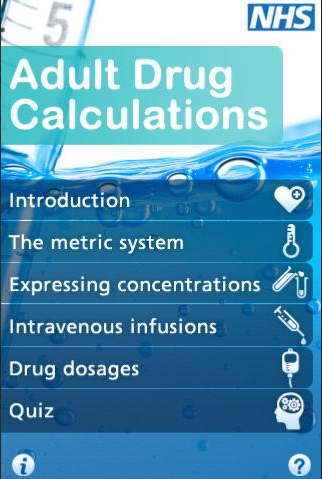
\includegraphics[width=\linewidth]{C:/Users/Nicole/Documents/GitHub/team-project/Dissertation/images/NHSDrugApp/NHSDrugApp2.png}
\endminipage\hfill
\minipage{0.32\textwidth}
  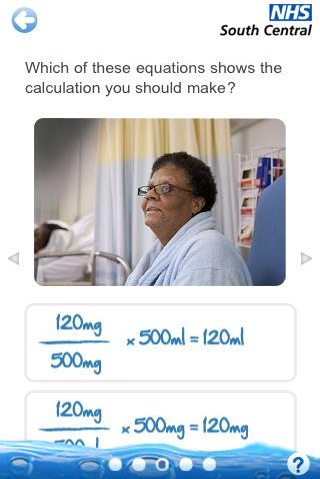
\includegraphics[width=\linewidth]{C:/Users/Nicole/Documents/GitHub/team-project/Dissertation/images/NHSDrugApp/NHSDrugApp4.png}
\endminipage
\end{figure}


The NHS Adult Drug Calculations, a smartphone based learning tool, allows the user to browse through different topics. Within each topic, there are a number of slides providing the user with the information and theory behind the calculations, and then has a few "Check your knowledge" slides containing multiple choice questions to test the user on what they have read. The interface is very simple and easy to use. The main menu allows the user to simply select which topic they qish to go over. Within each topic, there are arrows on each page which will allow the user to navigate back and forward between the pages and there are breadcrumbs at the bottom of each page indicating how far through the topic they are.  There is also an arrow at the top left-hand corner which will allow the user to return to the main menu at any point. One feature which is particularly useful to new users is the help button, which informs the user how to use the application. This application is very similar to the application which our client would like for the vetinary students.

\subsubsection{Vet Calculator}

\begin{figure}[!htb]
\minipage{0.32\textwidth}
  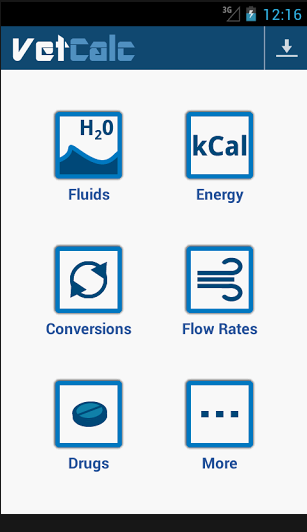
\includegraphics[width=\linewidth]{C:/Users/Nicole/Documents/GitHub/team-project/Dissertation/images/VetCalcApp/VetCalcApp1.png}
\endminipage\hfill
\minipage{0.32\textwidth}
  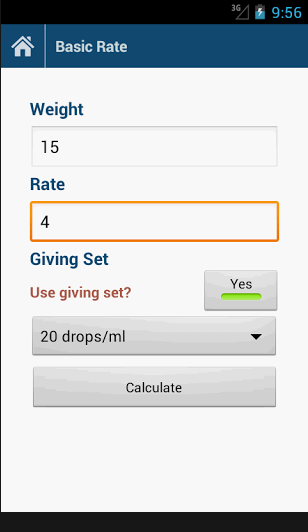
\includegraphics[width=\linewidth]{C:/Users/Nicole/Documents/GitHub/team-project/Dissertation/images/VetCalcApp/VetCalcApp3.png}
\endminipage\hfill
\minipage{0.32\textwidth}%
  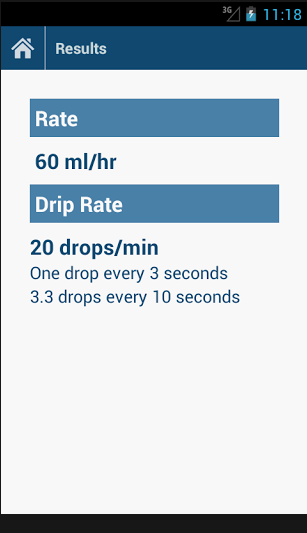
\includegraphics[width=\linewidth]{C:/Users/Nicole/Documents/GitHub/team-project/Dissertation/images/VetCalcApp/VetCalcApp4.png}
\endminipage
\end{figure}

VetCalc is an android based tool which allows the user to enter the necessary details, such as weight; dose; formulation; volume of fluid; etc. and will produce the result for the user. The interface for the vet calculator is very simple and easy to use. The menu is a simple grid-layout of different topics and sections for drug calculations. Within each topic, the user has to simply enter the necessary details into the clearly labelled text boxes and click 'Calculate' in order to get the result of the calcuation. On each page, there is a home button which will easily allow the user to return to the main menu at any point. This application is useful for users who simply need to get the results of a calculation. However, out client wants an application that will teach the students how to carry out the calculations and not simply produce the result for them as they will need to know how to carry out these calculations throughout their career.

\subsection{Revision Tools}

\subsubsection{Bitesize}

ROSS TO DO!

\subsubsection{Hot Potato}

ROSS TO DO!

\end{document}
